\documentclass[11pt]{article}
\usepackage{amsmath, amssymb, amscd, amsthm, amsfonts}
\usepackage{graphicx}
\usepackage{hyperref}

\oddsidemargin 0pt
\evensidemargin 0pt
\marginparwidth 0pt
\marginparsep 10pt
\topmargin 00pt
\headsep 0pt
\textheight 8.7in
\textwidth 6.65in
\linespread{1.2}


\title{\vspace{-80pt}Truckee River Flow}
\author{Ben Hammel}
\date{\today}

\begin{document}

\maketitle

\vspace{-20pt}
\begin{abstract}
\noindent
In this project, I fit a bayesian linear regression model to predict high-water or flood events from the Truckee river in Reno, NV.
\end{abstract}

\section{Introduction}
\label{S:1}

\begin{figure}[h]
\centering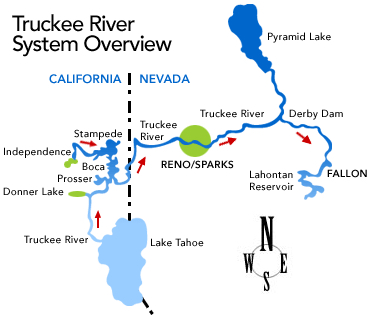
\includegraphics[width=.4\linewidth]{riversystem_map.jpg}
\caption{Truckee River System}
\label{Fig. 1}
\end{figure}
The Truckee River flows from Lake Tahoe, CA to Pyramid Lake, NV. The Truckee serves to provide drinking water for Reno, irrigation for farms in the Great Basin, and recreational use such as fishing or kayaking. In the winter and spring, snowmelt from the Sierra Nevada mountains and natural run-off feed the river. In the summer, the river's main water supply is maintained by releases from Lake Tahoe and surrounding reservoirs, seen in Figure \ref{Fig. 1}.

\section{Data}

We obtain data collected from the United States Geological Services \cite{U.S.G.S.:2019aa} and the National Center for Environmental Information \cite{Menne:2019aa} that we assume may impact water flow: 1) Output from surrounding lakes and reservoirs: Tahoe, Boca, Donner
2) Snowpack level 3)  Precipitation 4)Temperature.

\begin{figure}[h]
\centering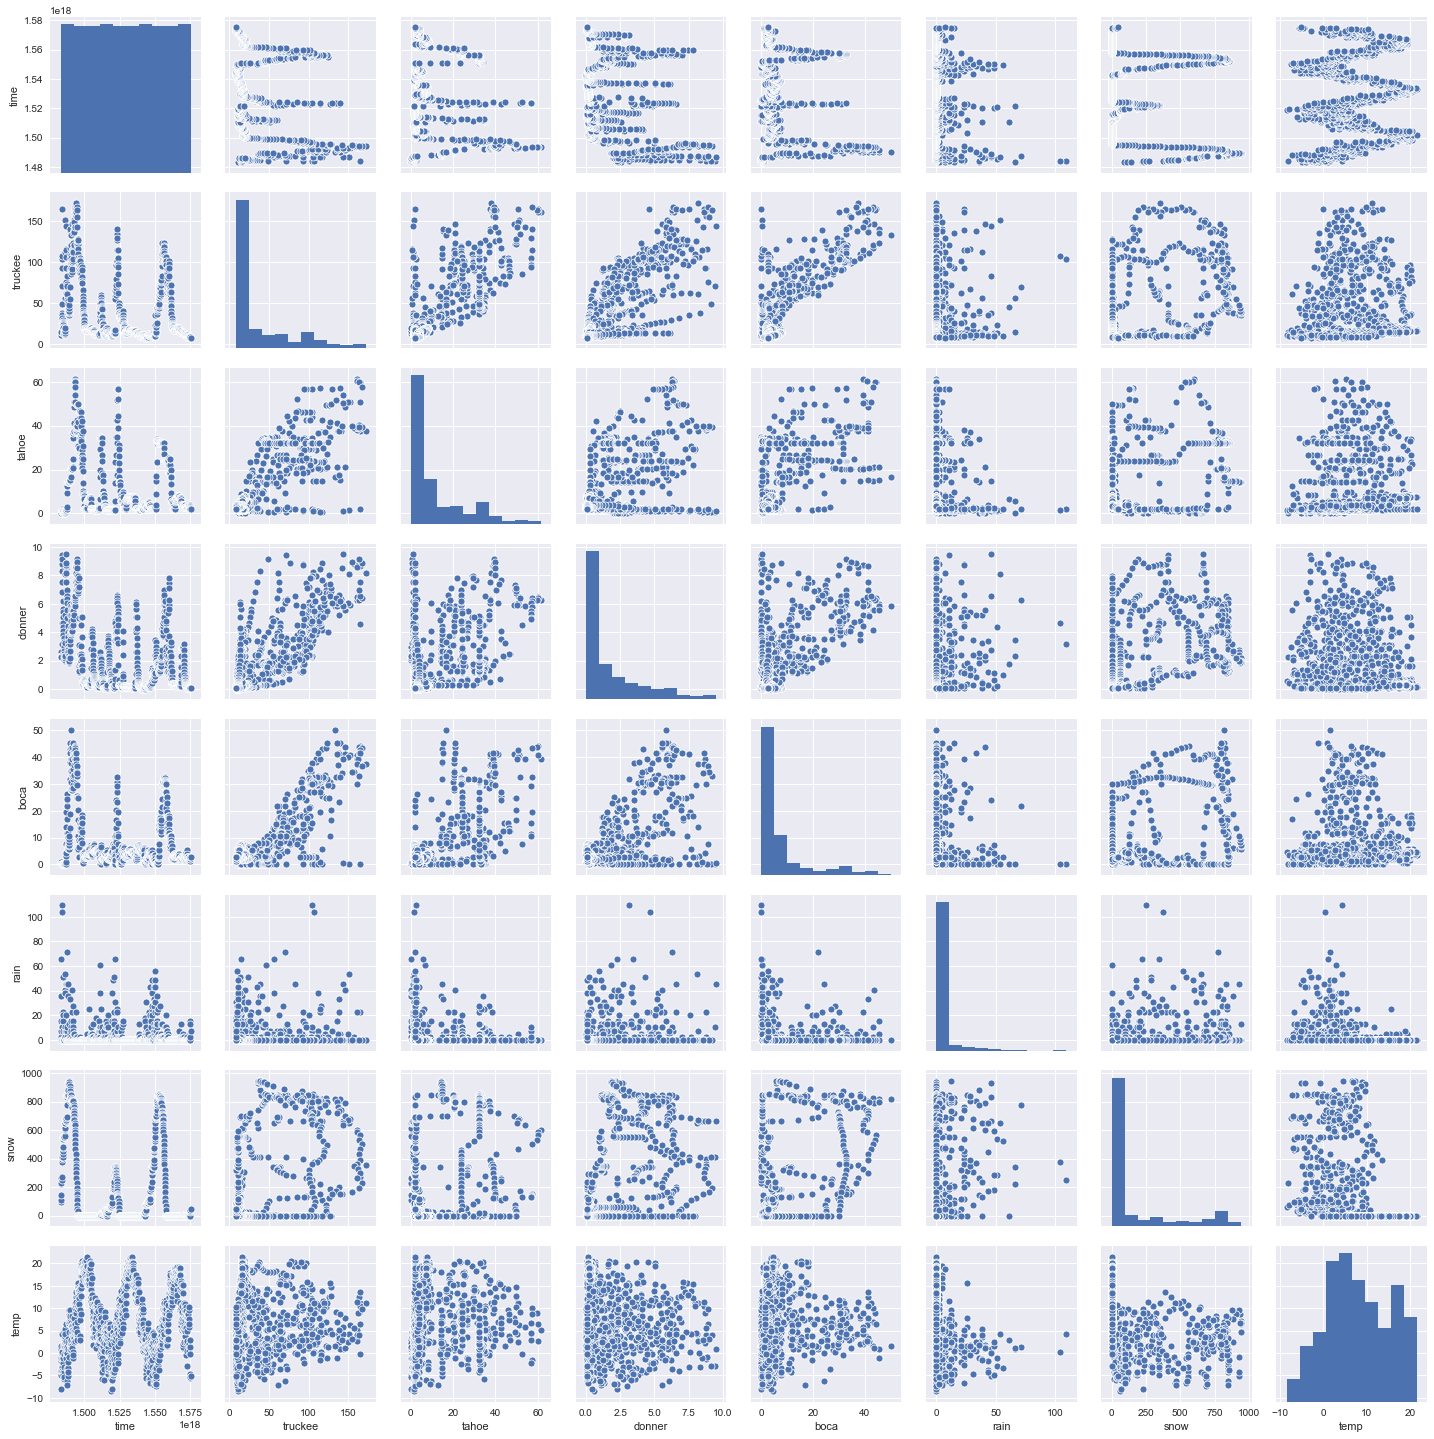
\includegraphics[width=.8\linewidth]{data.png}
\caption{Data}
\label{Fig. 2}
\end{figure}

The data is reported with a cadence of 1 day. We remove NAN values associated with sensors being down, and linearly interpolated between adjacent days to fill the missing values. After the data pre-processing \cite{github:aa}, we have over one-thousands consecutive days of information about water flow and environmental information. All units are converted to metric. Our predictive value, The Truckee water flow, is recorded by the USGS sensor located in Reno, NV.
Our assumptions on data importance is outlined below:

\begin{itemize}
\item Output from the lakes and reservoirs will have the strongest predictive ability on the Tuckee river flow
\item There may be times when output of feeder rivers decrease and the Truckee increases. This could be in cases of rapid snowmelt events.
\item Snowpack serves as a signification storage of water during the winter and can rapidly flood the Truckee in the springtime. For this reason, we use the ``Snow Water Equivalent" (SWE) metric as opposed to "Snow Pack Depth." SWE is the theoretical water volume obtained if the snowpack were to be instantaneously melted.  It includes additional factors such as snow density, which are not represented in snow pack depth.
\item Precipitation can either contribute linearly to, contribute non-linearly to,  or not contribute at all to river levels. If the temperature is low, precipitation will fall as snow and add to the snowpack, not river volume. In the summer, when temperatures are high, rainfall will directly add to the river water volume. However, In the spring, rainfall will rapidly melt the snowpack and create the high-water events we want to predict.
\end{itemize}

\noindent
For initial simplicity, we do not try to model the cross terms e.g. water contribution due to precipitation, temperature, and snow water equivalent. Instead, we use the feature $  d {\rm SWE} / dt $ in the model. This feature has more of a direct relation with river output, but has the disadvantage that this value needs to be inferred from a separate predicted model. We do not discuss this separate model in this write-up, instead we assume we have an appropriate model to use.

\section{Model}

The initial model we fit is:

$$
y(t_i) = \beta_0 I_{\rm Boca} (t_i) + \beta_1 I_{\rm Tahoe} (t_i) + \beta_2 I_{\rm Donner} (t_i) + \beta_3 \frac{1}{n} \sum_{j{=}0}^n  \frac{d {\rm S(t_{i-j})}}{dt} + \beta_4  \frac{1}{n} \sum_{j{=}0}^n R(t_{i - j}).
$$

\noindent
Wherein, $I_{\rm River}$ is the input river flow, $\sum dS/dt$ is the average change in snowpack, and $\sum R$ is average rainfall. The number of days to average over is a hyperparameter and was hand tuned, for this work $n$ was set to 5. The Gelman–Rubin diagnostic along with the trace plots indicate we've converged and reached equilibrium. Inferred coefficients are given in the table below:
 

\begin{center}
\begin{tabular}{ |p{2cm}||p{1.5cm}|p{1.5cm}|p{1.5cm}|p{1.5cm}|p{1.5cm}|p{1.5cm}|p{1.5cm}|  }
 \hline
 \multicolumn{8}{|c|}{Inference Coefficients} \\
 \hline
 Coefficient & mean & std & median & 5.0\% & 95.0\% & $n_{\rm eff}$ & $r_{\rm hat}$ \\
 \hline
$\beta_0$  &   1.21  &   0.05  &   1.21  &   1.13  &   1.29 &  14248.90  &   1.00 \\
$\beta_1$  &   1.17  &   0.03  &   1.17  &   1.12  &   1.22 &  16062.51  &   1.00 \\
$\beta_2$  &   5.05  &   0.21  &   5.05  &   4.70  &   5.37 &  14785.20  &   1.00 \\
$\beta_3$  &  -0.66  &   0.06  &  -0.66  &  -0.76  &  -0.57 &  11687.75  &   1.00 \\
$\beta_4$  &   1.02  &   0.06  &   1.02  &   0.92  &   1.12 &  10728.03  &   1.00 \\
$\beta_5$  &   2.92  &   0.47  &   2.92  &   2.14  &   3.68 &  16223.93  &   1.00 \\
std        &  10.36  &   0.22  &  10.35  &  10.00  &  10.73 &  16924.01  &   1.00 \\
 \hline
\end{tabular}
\end{center}

It is surprising to see the coefficient $\beta_2$ - for the input river from Donner Lake - have a value much different than 1. We expect this number to be closer to 1 because conservation of mass tells us inputs should be equal to the output. We are left to assume that the additional water volume is due to surrounding unmonitored streams. We initially hoped that unmonitored stream behavior would be captured by the rain fall feature, however there seems to be too much variability in this feature to be a strong predictor. We try to fit another simpler model which uses the sum of the input rivers as a single feature.

$$
y(t_i) = \beta_0 \sum I(t_i) + \beta_1 \frac{1}{n} \sum_{j{=}0}^n  \frac{d {\rm S(t_{i-j})}}{dt} + \beta_2  \frac{1}{n} \sum_{j{=}0}^n R(t_{i - j}).
$$

\noindent
However, the DIC metric indicates a strong preference for our original model.

\section{Results}

\begin{figure}[h]
\centering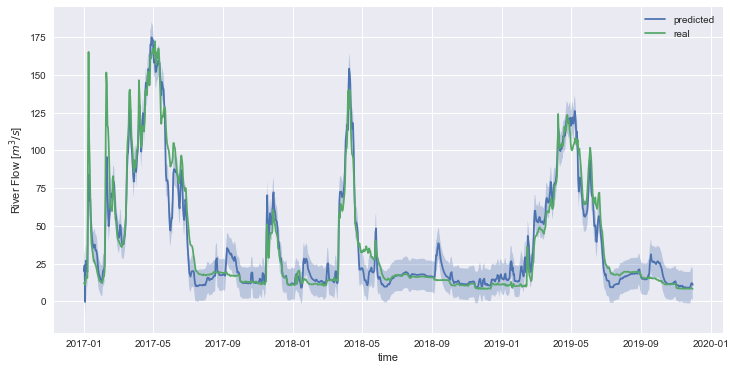
\includegraphics[width=\linewidth]{flow.png}
\caption{Predicted river flow}
\label{Fig. 4}
\end{figure}

To demonstrate our model we ask the following question: given the information we had, what was the probability of the 2017, January 10th flood event occurring? We find that our model predicts the probability of flow in the Truckee being greater than 150 $m^3/s$, given the initial conditions, to be 2\%. 

\section{Conclusions}

We have been able to build a strong baseline for predicting water flow in the Truckee river. Our model can provide probabilistic predictions to inform us of high-water events; however, future work is needed to more precisely predict rare flood events. Furthermore, future work should explore the ability to incorporate snowpack as a predictive feature, as opposed to relying on an external predictive model to estimate the change in snowpack due to temperature and rain fall.

\bibliographystyle{abbrv}
\bibliography{refs}

\end{document}
